\begin{figure*}[hbtp]
  \centering
  \subfigure[Overall result]{
    \label{fig:8020-runtime--mean}
    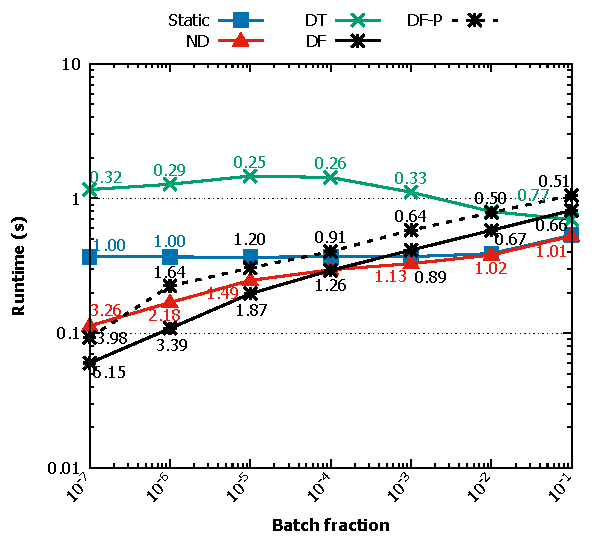
\includegraphics[width=0.38\linewidth]{out/8020-runtime-mean.pdf}
  }
  \subfigure[Results on each graph]{
    \label{fig:8020-runtime--all}
    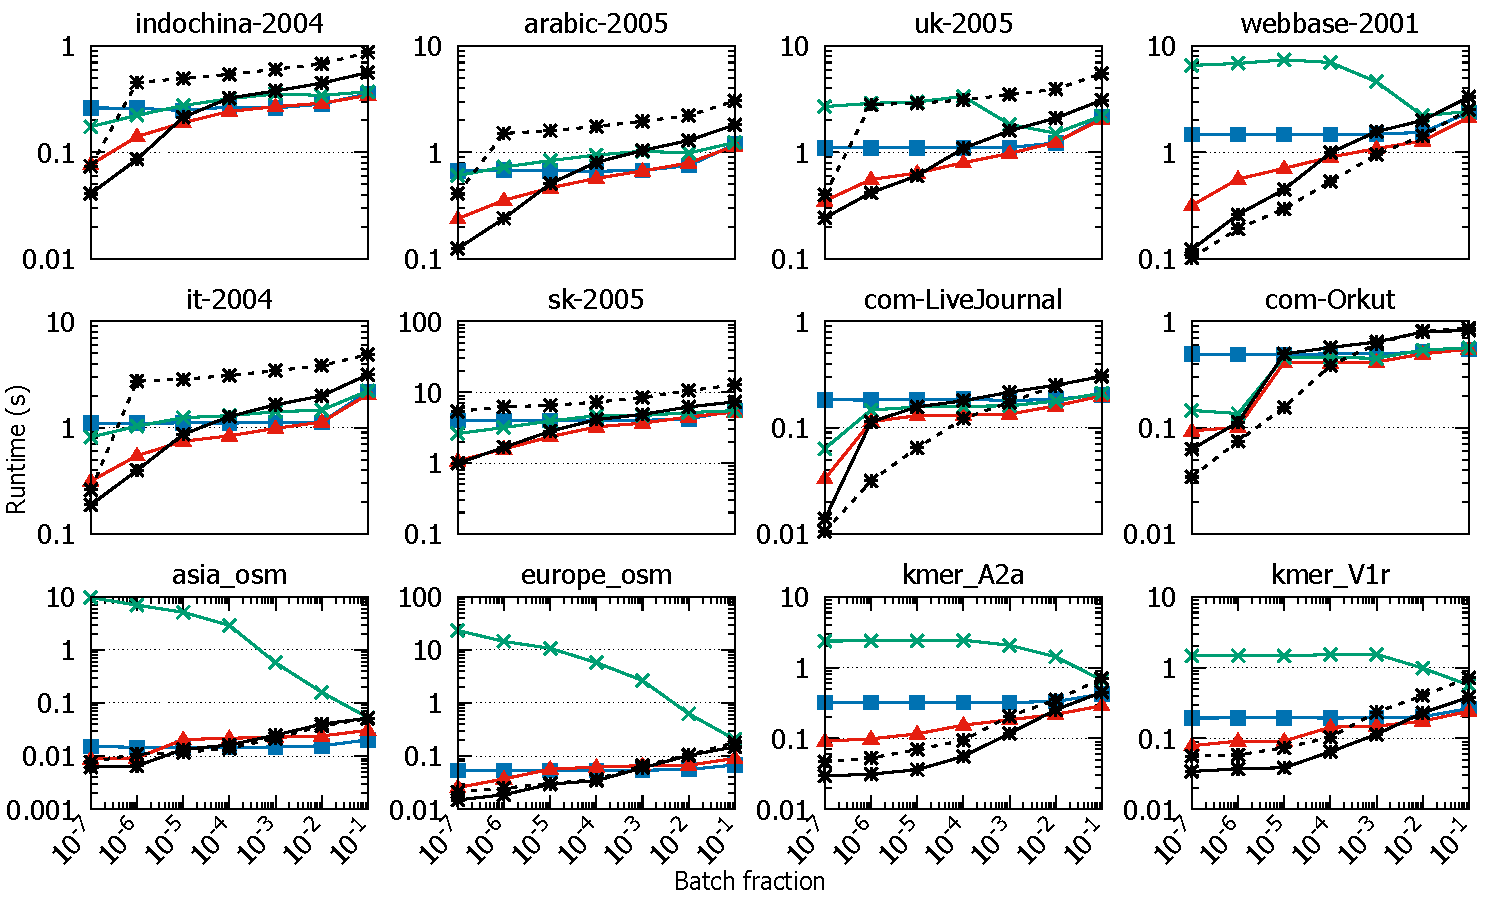
\includegraphics[width=0.58\linewidth]{out/8020-runtime-all.pdf}
  } \\[-1ex]
  \caption{Runtime (logarithmic scale) of \textit{Static}, \textit{Naive-dynamic (ND)}, \textit{Dynamic Traversal (DT)}, our improved \textit{Dynamic Frontier (DF)}, and \textit{Dynamic Frontier with Pruning (DF-P)} PageRank on large (static) graphs with generated random batch updates, on batch updates of size $10^{-7}|E|$ to $0.1|E|$ in multiples of $10$. The updates include $80\%$ edge insertions and $20\%$ edge deletions, simulating realistic changes upon a dynamic graph. The subfigure on the right illustrates the runtime of each approach for each graph in the dataset, while the subfigure of the left presents overall runtimes (using geometric mean for consistent scaling across graphs). In addition, the speedup of each approach, relative to Static PageRank, is labeled on respective lines.}
  \label{fig:8020-runtime}
\end{figure*}
